\documentclass[aspectratio=169]{beamer}
\usetheme{Madrid}
\usecolortheme{beaver}
\usepackage[utf8]{inputenc}
\usepackage[T1]{fontenc}
\usepackage{tikz}
\usepackage{amssymb}
\usepackage{graphicx}
\setbeamertemplate{navigation symbols}{}
\setbeamercolor{title}{fg=white,bg=blue!55!black}
\setbeamercolor{frametitle}{fg=white,bg=blue!45!black}
\setbeamercolor{block title}{bg=blue!15,fg=black}
\setbeamercolor{block body}{bg=blue!5,fg=black}

\title{Web Story 1 — Remembering the Reader}
\subtitle{Arrays and objects — a story that tracks the reader's inventory and flags}
\author{ByteForge --- Grade 8 --- App Builder}
\date{}

\begin{document}

\begin{frame}
    \titlepage
\end{frame}

\begin{frame}{Today's Plan}
    \begin{itemize}
        \item Your First Array
        \item Add to the Array
        \item A Flag Object
        \item[$\bigstar$] BOSS --- Inventory \& Flags Together
    \end{itemize}
\end{frame}

\begin{frame}{An array is an ordered list of values}
    \Large
    \texttt{["sword", "shield"]} is a genuine JavaScript array — an ordered collection, indexed from 0. \texttt{.join(", ")} turns it back into one readable string.

    \begin{center}
    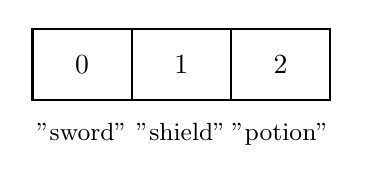
\begin{tikzpicture}[scale=0.9]

        \draw[thick] (0,0) rectangle (1.4,-1); \node at (0.7,-0.5) {0};
        \draw[thick] (1.4,0) rectangle (2.8,-1); \node at (2.1,-0.5) {1};
        \draw[thick] (2.8,0) rectangle (4.2,-1); \node at (3.5,-0.5) {2};
        \node[below] at (0.7,-1.2) {\small "sword"};
        \node[below] at (2.1,-1.2) {\small "shield"};
        \node[below] at (3.5,-1.2) {\small "potion"};
    \end{tikzpicture}
    \end{center}
\end{frame}

\begin{frame}{An array is an ordered list of values --- Worked Example}
    \Large
    Worked example: \texttt{["sword","shield"].join(", ")} produces the exact text "sword, shield" — this is genuinely how a real inventory line of text gets built from structured data.
\end{frame}


\begin{frame}{.push() adds to the END of an array}
    \Large
    An array isn't fixed once written — \texttt{.push("potion")} genuinely adds a new element after the array already exists, exactly like a player finding a new item mid-story.
\end{frame}


\begin{frame}{An object groups related NAMED values}
    \Large
    An array is a list, ordered by position; an object is a set of NAMED properties (\texttt{flags.hasKey}) — both are "collections" but answer different questions.
\end{frame}


\begin{frame}{BOSS — arrays and objects, together}
    \Large
    An inventory (an ordered LIST) and a set of flags (NAMED yes/no facts) are genuinely different shapes of data — a real interactive story needs both.
\end{frame}

\begin{frame}{Real-World Example}
    \Large
    Every real e-commerce cart is an array of items plus a set of named flags ("giftWrapped", "expressShipping") — exactly this chapter's two data shapes, doing real work. Minecraft's own inventory (an ordered list of slots) plus achievement flags (has this player found diamonds yet?) is the same split.
\end{frame}


\begin{frame}{Image}
    \begin{center}
    
\includegraphics[width=0.5\textwidth]{images/js.png}

    \large Real JavaScript --- the language behind this week's arrays and objects.

    \small JavaScript logo — Chris Williams, public domain, via Wikimedia Commons
    \end{center}
\end{frame}

\begin{frame}{Let Them Discover}
    \Large
    Open your phone's shopping app cart. Is the item list ordered (an array) or does order not matter? Now think of one yes/no fact the app tracks about you (signed in? has a coupon?) — that's an object property.
\end{frame}

\begin{frame}{Your Turn}
    \Large
    Open the student map, find \textbf{Web Story 1 — Remembering the Reader}, and work through it
    hands-on --- everything you just saw, they now do themselves.
\end{frame}

\end{document}
